\documentclass[11pt,letter]{article}
\usepackage[top=1.00in, bottom=1.0in, left=1.1in, right=1.1in]{geometry}
\renewcommand{\baselinestretch}{1.1}
\usepackage{graphicx}
\usepackage{natbib}
\usepackage{amsmath}
\usepackage{amssymb} 
\usepackage{hyperref} 

\def\labelitemi{--}
\parindent=0pt
\begin{document}

\title{The illusion of declining temperature sensitivity with warming OR A simple explanation for declining temperature sensitivity with warming} % Sensitivities are not declining with warming OR As climate change accelerates biology, chasing statistical artifacts ensues
\author{E. M. Wolkovich$^{1,a}$, C. J. Chamberlain$^{2}$, D. M. Buonaiuto$^{2}$, \\ A. K. Ettinger$^3$, I. Morales-Castilla$^{4}$ [Auerbach \& Gelman]} % Order is JUST alphabetical right now, not set.

\date{\today} 
\maketitle
**Authorship order is not set.\\
$^1$Forest \& Conservation Sciences, Faculty of Forestry, University of British Columbia, Vancouver, British Columbia, Canada\\
$^2$Department of Organismic and Evolutionary Biology, Harvard University, Cambridge, Massachusetts, USA\\
$^3$TNC, USA\\
$^4$Department of Life Sciences, University of Alcal\`a CTRA N-II, KM., 33,600, 28802, Alcal\`a de Henares, Spain\\
$^a$Corresponding author.

\section{Main text}
\begin{abstract}
The concept of temperature sensitivity is fundamental to many disciplines, especially in biology, where temperature determines the rate of diverse plant, animal and ecosystem processes. Recently, a growing body of literature has found declining temperature sensitivities with global warming \citep{fu2015,gusewell2017,dai2019ag}. Such declines are predicted if warming causes fundamental shifts in underlying biological processes, but to date researchers have not conclusively documented changes in the underlying biology. Here we show a far more simple explanation for observed declining sensitivities: the use of linear methods to describe non-linear temperature responses. Simple corrections for the non-linearity of temperature response in simulated (and probably real---working on that) data remove the apparent decline. By accelerating biological time climate change thus makes methods and approaches that may work in stationary systems problematic for inferring mechanism from measurements today.
\end{abstract}

Climate change has already reshaped biological processes around the globe, with shifts in the timing of major life history events (phenology), in carbon dynamics and other ecosystem processes \citep{IPCC:2014sm}. With increasing warming,  a growing body of literature has documented a suite of changes in temperature sensitivity---the magnitude of a response scaled per $^{\circ}$C---including apparently declining responses to temperature in recent decades \citep{fu2015,gusewell2017,piao2017,dai2019ag}, and more uniform sensitivities across elevation \citep{vitasse2018}. Researchers generally suggest these shifts in temperature sensitivity are driven by fundamental shifts in underlying biological processes. For example, fundamental science suggests that warm temperatures (`forcing') are the main controller on many temperate phenological events (e.g., leafout, insect emergence), but cool temperatures (referred to often as `chilling' and generally associated with dormancy processes) or photoperiod can also play a role, especially given warmer winters. Thus, observed declines in the temperature sensitivity of temperate plant phenology with warming are generally attributed to the increasing role of photoperiod or chilling  \citep[e.g.,][]{fu2015,gauzere2019}. Yet, providing strong evidence of this mechanistic link is difficult given that the underlying model of exactly how these other factors control phenological events is unknown \citep{chuine2016}, and that the cues are generally correlated in nature given long-term trends in warming \citep[e.g.,][]{fu2015}. \\
% ... fundamental science predicts declines in the temperature sensitivity of temperate plant phenology, as the role of spring temperature diminishes relative to the increasing importance of winter temperatures and daylength % For example, the temperature sensitivity of spring leafout may decline if warmer winters mean plants fail to receive enough winter chilling.  


% Given the difficulty of providing strong evidence that shifting biology underlies shifting temperature sensitivities, a small but increasing number of studies have focused on potential issues---shifts in temperature variance and complexities in defining relevant temporal windows---in commonly used metrics of temperature sensitivity.
Given the difficulty of providing strong evidence that shifting biology underlies shifting temperature sensitivities, a small but increasing number of studies have focused on potential statistical issues with commonly used metrics of temperature sensitivity. Studies to date have shown how shifts in temperature variance and related complexities in defining relevant temporal windows \citep{clark2014a,gusewell2017,keenan2019} can influence estimated sensitivities, but have not explained observed shifts. Importantly, all have examined sensitivities through methods based on assumptions of linearity, ignoring that many biological processes to temperature are non-linear. \\

Metrics of temperature sensitivity focused on shifting responses generally rely on some form of linear regression to compute a change in a quantity---days to leafout or carbon sequestered, for example---per $^{\circ}$C. Many observed biological events, however, are the result of continuous processes that depend on temperature which are discretized into temporal units for measurement. Leafout, for example, is generally observable only after a certain thermal sum is reached, and plants will reach this threshold more quickly---in calendar time---when average daily temperatures are, for example, 15$^{\circ}$C compared to when they are 10$^{\circ}$C. Biologically, however, the plants require the exact same temperature sum and have not shifted their sensitivity to temperature. Indeed any process observed or measured as the time until reaching a threshold is inversely proportional to the speed at which that threshold is approached. Thus, at very low temperatures plants would never leaf out and at higher temperatures they could leaf out in only a matter of days---and sensitivities estimated from simple linear regression at these higher temperatures would appear much lower than those observed at lower temperatures (given the low variance possible for response variable). Warming acts to step on the biological accelerator, and makes the use of classic calendar time precarious. \\
% calendar time is the same, but the biological time is much greater
% amount of change that can occur in a day depends on temperature

Simple simulations of biological events observed after a certain thermal sum show that sensitivities estimated from simple linear regression will always appear to decline with warming (Fig. \ref{fig:basicsims}, code link). Examining the same responses using proportional change or logged variables removes the apparent decline, and yields a constant sensitivity of 1 \citep[the expected slope given that these sensitivities are effectively include temperature as both the predictor and response variable, ][]{nee2005}. Using alternative simulations where warming increases the required thermal sum for a biological event---a common hypothesis for declining sensitivities in spring phenological events---show declining sensitivities that cannot be corrected by adjusting response variables using proportions or logs (Fig. \ref{fig:biosims}) \\

[Here we add what we see with the PEP 725 data.] \\

Inferring biological processes from statistical artifacts is not a new problem \citep[e.g.,][]{nee2005}, but climate change provides a new challenge in discerning mechanism from measurements because it accelerates biological time over years and reshapes the spatial landscape of temperature. Before anthropogenic climate change, the use of sensitivities calculated from linear models may have been less prone to yielding notable temporal patterns. With warming declining sensitivities with higher warming should be the null model for analyses using simple linear regressions, and highlights how the nonstationarity of climate change upends methods and approaches that may work in stationary systems \citep{Milly:2008yu,tempeco}.  Attempts to use sensitivities to identify shifting biological process across space has always required caution \citep[e.g.,][]{Phillimore2012,tansey2017}, but climate change adds further complexity. \\

Research inferring biological processes from differing temperature sensitivities across space and time must look beyond shifting sensitivities with warming as strong evidence. Other fields, focused on temperature sensitivity generally use approaches that avoid the issue we have outlined here, such as the use of $Q_{10}$ in soil science. Researchers have called for more use of process-based models \citep{keenan2019}, which is also beneficial. But many fields, still lack the underlying mechanistic understanding to robustly develop and fit process-based models, and thus many parameters and exact model specification are still unknown \citep{chuine2016}. Thus using more exploratory methods will remain necessary to advance science, but findings from such methods must be interrogated vigorously, confronted with multiple diverse methods of calculating similar metrics, and tested for logical outcomes.Greater use of data simulation and null models is can highlight issues and force greater focus on mechanisms. 
% Process-based models can help some, but are not an obvious solution given gaps in our understanding that make parameter estimation difficult. We say process models are good, but not the whole answer. Instead we need more people to simulate process and stats and see what the hell they're doing... try lots of methods.

\emph{Acknowledgements:} Thanks to TMG, TJD and others. 

\bibliographystyle{..//refs/bibstyles/amnat.bst}
\bibliography{..//refs/decsens.bib}

\section{Outline \& notes}

Need to work on this, notes to date on \href{https://github.com/lizzieinvancouver/decsens/wiki/Statistical-artifacts-in-sensitivities}{here}.\\

\emph{Meeting with Jonathan Auerbach \& Andrew Gelman on 18 December 2019:} 

Fundamental issue is that we have a non-linear relationship ($y=1/x$) being described by a linear function ($y=x$), where $x$ is the mean temp and 1 could be the GDD. The time until you reach a threshold is inversely proportional to the speed you go at. So, at very low temperatures plants would (theoretically) never leaf out and at 200 C days it would take one day. \\

The classic algebra example (they tell me) is how long does it take to drive 200 miles? It depends on your miles per hour. (Side note by Lizzie while typing up these notes: the speed analogy is sort of nice, climate change is stepping on the accelerator, making this algebra problem relevant.)

\begin{itemize}
\item The artifact comes from the mean getting larger while the variance goes down (I think, I may have this noted wrong, but it's about the mean relative to the variance, not just the variance or the mean). If you make the variance scale with the mean you will see the issue go away (though Andrew pointed out this should be done on the $SD$ scale, not the $var$).
\item ``The statistical artifact is that fitting a linear regression requires linearity''said  Jonathan Auerbach.
\item If this was all simple, we could fix it two ways: percent scale (decline relative to some base C temp) or log both axes. (Note from Lizzie: but we don't know when to start accumulating so not sure how this works, though Jonathan seemed to have insight into this.)
\item An example of inferring process from an artifact is regression to the mean, though Andrew pointed out regression to the mean is more complicated compared to this as regression to the mean is a statistical issue and this is just a deterministic reality. 
\item Convexity in economics has had similar problems to this. 
\end{itemize}

\section{Tasks, milestones etc.}
\begin{itemize}
\item Finish minimal analyses we think we need:
\begin{itemize}
\item Produce simulated data where chilling is not met (Lizzie has notes on this below enddocument command ... (bucket model).
\item Do sliding windows for ... BETPEN (done) and FAGSYL from PEP725 and for simulated data.
\end{itemize}
\item Chat with Rob Guy for foundational papers that many events like leafout are based on temperature accumulations. 
\item Review the literature
\begin{itemize}
\item Cat did some of this: see \verb|ospree/analyses/bb_analysis/pep_sims/pepsimslitreview.txt|
\item Review beyond phenology?
\end{itemize}
\item Outline the paper
\item Decide on targeted journals
\item Write the paper
\item Submit the paper
\end{itemize}

\section{Literature notes}


Sagarin 2001: False estimates of the advance of spring (leap year issues). \\

I noticed as you go back to 2014 and before in my ISI searches, you get a lot of soil respiration lit. And in that literature they use $Q_{10}$ for temperature sensitivities, ``[t]he temperature sensitivity of soil respiration is often expressed as the Q10 value; that is, the factor by which soil respiration increases by a 10°C increase in temperature (e.g., Kirschbaum, 1995; Van't Hoff, 1898),'' which would avoid a good dose of the issue we're seeing.\\  % definition from https://agupubs.onlinelibrary.wiley.com/doi/full/10.1002/2017GB005644
% Van't Hoff, J. H. (1898). Lectures on theoretical and physical chemistry. In Chemical Dynamics Part I (pp. 224–229). London: Edward Arnold.

Shen et al. 2014 shows earlier-season vegetation more temperature-sensitive, which is the same artifact. Do we want to work this in?

\section* {Figures}

\begin{figure}[h!]
\centering
\noindent 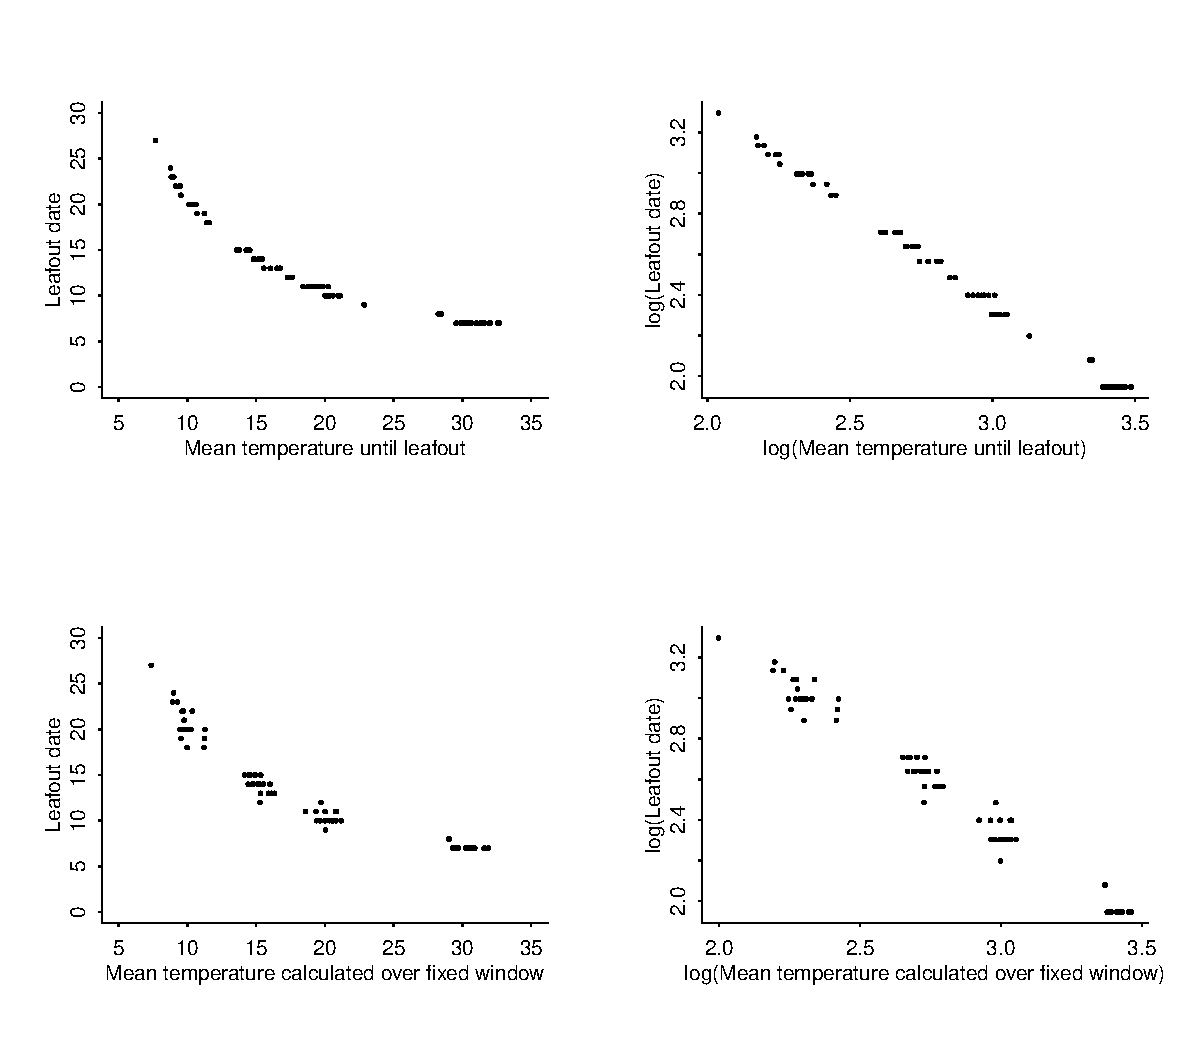
\includegraphics[width=1\textwidth]{..//analyses/figures/simslogging.pdf}
\caption{\textbf{Simulated leafout as a function of temperature across different temperatures highlights non-linearity of process.} Here we simulated sets of data where leafout constantly occurs at 200 growing degree days across mean temperatures of 0, 5, 10 and 20C (constant SD of 4), we calculated estimated mean temperature across a fixed window (top row, similar to estimates of 'spring temperature') or until leafout date (bottom row). While within any small temperature range the relationship may appear linear, is non-linear relationship becomes clear across the range shown here (left). Taking the log of leafout (middle) reduces this some, but taking the log of both leafout and temperature (right) linearized the relationship.}
\label{fig:simslog} % decsensSimsAuerbach.R
\end{figure}



\begin{figure}[h!]
\centering
\noindent 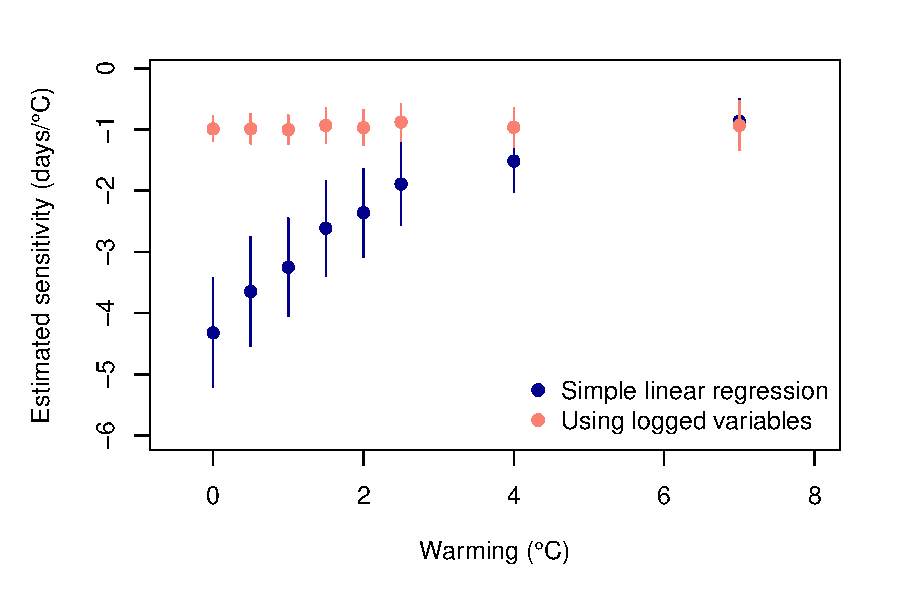
\includegraphics[width=0.75\textwidth]{..//analyses/figures/basicsims.pdf}
\caption{\textbf{Declining sensitivities with warming explained by using linear regression for non-linear processes.} We found declines in estimated sensitivities with warming from simulations with no underlying change in the biological process when sensitivities were estimated with simple linear regression (``Simple linear regressions''). This spurious decline can be removed by performing the regression on logged predictor and response variables (``Using logged variables'').}
\label{fig:basicsims} % decsensSims.R
\end{figure}


\begin{figure}[h!]
\centering
\noindent 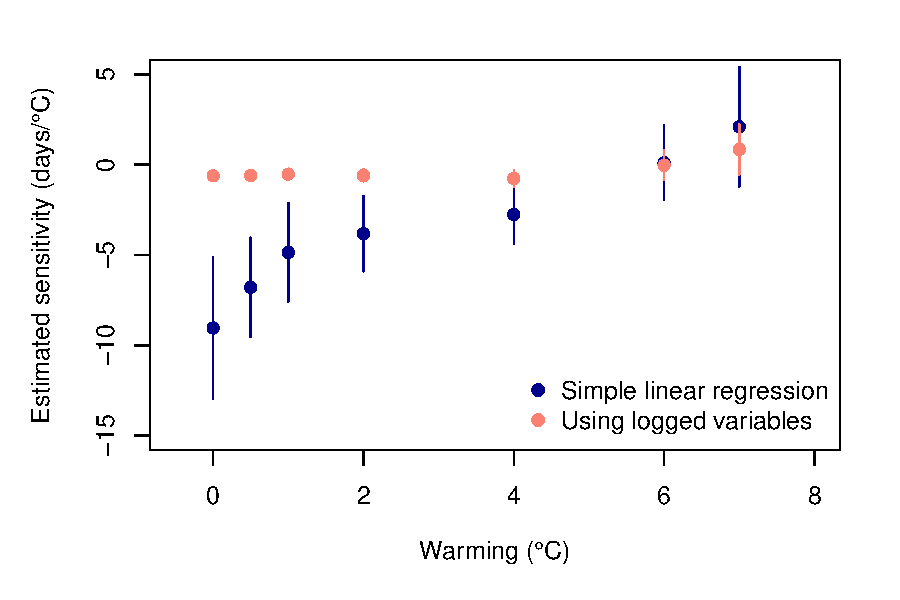
\includegraphics[width=0.75\textwidth]{..//analyses/figures/shiftingcuessims.pdf}
\caption{\textbf{Truly declining sensitivities remain even after correction.} Here we used simulations where the biological process shifts at moderate warming levels (basically I made the GDD increase when chilling was low, see the code). }
\label{fig:biosims} % decsensSimsMo.R
\end{figure}


\begin{figure}[h!]
\centering
\noindent 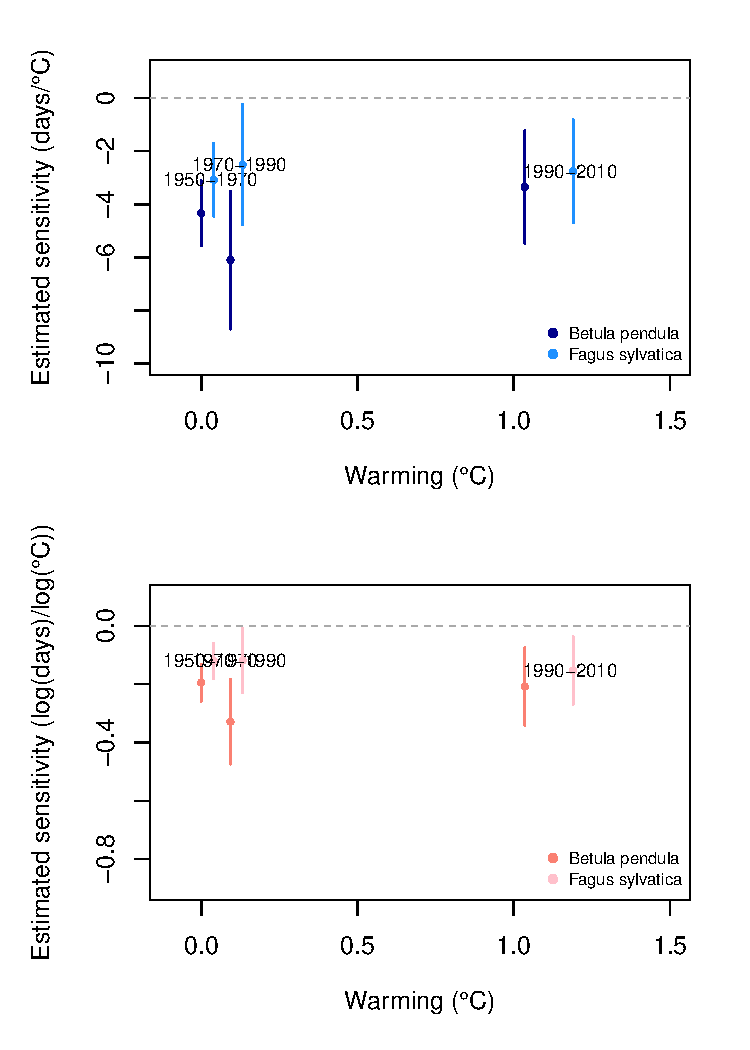
\includegraphics[width=0.75\textwidth]{..//analyses/figures/basicpep1950to20002spp2panel.pdf}
\caption{\textbf{Sensitivities for two species from PEP725 data} using raw data (top) or logged variables (bottom) using 20 year windows of data (lines show 78\% confidence intervals). Amounts of warming are calculated relative to 1950-1970 and we used only sites with leafout data in all years shown here. Both approaches show variation in sensitivity across time. To aid visualization \emph{Fagus sylvatica} are jittered slightly to the right, but warming is approximatly 0.08 C greater for \emph{Fagus sylvatica} in 1990-2010 relative to \emph{Betula pendula}.}
\label{fig:pepper} % pepplotting.R
\end{figure}


\end{document}

Simulate bucket model task

Weather first (1-5), then phenology (6-7):
1. Skip fall
2. Simulate stochastic stationary, cold winter (make sure this hits too little chill at some level of warming)
3. Simulate stochastic stationary, warm spring
4. Build transition between 3 and 4.
5. Do warming as we have -- add 1:7 degrees
6. Calculate GDD (1 Jan onward) and chilling (1 Nov - 1 Feb)
7. Select some range of high chill where same GDD is needed for budburst, then set up a linear relationship between chill (at lower range) and GDD required (more GDD for lower chill)
8. Predict GDD based on simulated weather and 7.

\begin{align*}
y_i &= \alpha_{sp[i]} + \beta_{forcing_{sp[i]}} + \beta_{photoperiod_{sp[i]}} + \beta_{chilling_{sp[i]}} + \beta_{latitude_{sp[i]}} + \beta_{photoperiod x latitude_{sp[i]}} + \epsilon{_i},\\
\epsilon_i \sim N(0,\sigma^2_y)
\end{align*}

This would be better .., 

\begin{align*}
y_i &= \alpha_{sp[i]} + \beta_{forcing_{sp[i]}} + \beta_{photoperiod_{sp[i]}} + \beta_{chilling_{sp[i]}} + \beta_{latitude_{sp[i]}} + \beta_{photoperiod x latitude_{sp[i]}} + \epsilon{_i},\\
& \epsilon_i \sim N(0,\sigma^2_y)
\end{align*}

or ...

\begin{align*}
y_i &= \alpha_{sp[i]} + \beta_{forcing_{sp[i]}} + \beta_{photoperiod_{sp[i]}} + \beta_{chilling_{sp[i]}} + \\
& \beta_{latitude_{sp[i]}} + \beta_{photoperiod x latitude_{sp[i]}} + \epsilon{_i}, \epsilon_i \sim N(0,\sigma^2_y)
\end{align*}


% \bibliography{..//..//refs/ospreebibplus.bib}
